\documentclass[10pt]{beamer}

\usetheme{metropolis}
\usepackage{appendixnumberbeamer}

\usepackage{booktabs}
\usepackage[scale=2]{ccicons}

\usepackage{pgfplots}
\usepgfplotslibrary{dateplot}

\usepackage{xspace}

\usepackage{tikz}
	\usetikzlibrary{shapes.geometric, arrows, positioning}
	\tikzstyle{startstop} = [rectangle, rounded corners, minimum width=3cm, minimum 		height=1cm,text centered, draw=black, fill=red!30]
	\tikzstyle{io} = [trapezium, trapezium left angle=70, trapezium right angle=110, minimum width=3cm, minimum height=1cm, text centered, draw=black, fill=blue!30]
	\tikzstyle{process} = [rectangle, minimum width=3cm, minimum height=1cm, text centered, draw=black, fill=orange!30]
\tikzstyle{decision} = [diamond, minimum width=3cm, minimum height=1cm, text centered, draw=black, fill=green!30]
\tikzstyle{arrow} = [thick,->,>=stealth]
\tikzstyle{arrow} = [thick,->,>=stealth]
%\usepackage{listings}
\usepackage{minted}

\usepackage{bm}%................................. Bold math symbols (after fonts)

\setbeamercolor{normal text}{bg=white}





\title{EML4930/EML6934: Lecture 12}
\subtitle{Scikit-Learn: Machine learning and \textbf{Regression}}
\date{November 16, 2017}
%\author{CJ}
\author{Charles Jekel}
%\titlegraphic{\includegraphics{images/avatarCropped.png}\vspace{58cm}}
%\institute{1. University of Florida\\ 2. Stellenbosch University, South Africa}

% \titlegraphic{\hfill\includegraphics[height=1.5cm]{logo.pdf}}

\begin{document}

\maketitle

\begin{frame}{More with Scikit-Learn}
\begin{itemize}
\item Saving Python objects with Pickle
\item Saving Scikit-Learn models with joblib
\item Cross Validation
\item Neural Network Example 
\end{itemize}
\end{frame}

\begin{frame}[fragile]{Saving Python objects with Pickle}
\begin{minted}
{python}
# This code fits a support vector classifier to the iris dataset
from sklearn import svm
from sklearn import datasets
clf = svm.SVC()
iris = datasets.load_iris()
X, y = iris.data, iris.target
clf.fit(X, y)  

# we can use Python's pickle to save the clf object
# pickle writes an object's memory state
import pickle
# save the clf object to 'my_svc_clf.p'
pickle.dump( clf, open('my_svc_clf.p', 'wb'))

# load clf object using
clf = pickle.load( open('my_svc_clf.p', 'rb'))

\end{minted}
\end{frame}

\begin{frame}[fragile]{You should use cPickle in Python 2}
In Python 2 you should use cPickle which is up to 1000 time faster than pickle. Python 3 automatically uses cPickle (if available). 
\begin{minted}
{python}
# importing from cPickle in Python 2
import cPickle as pickle
\end{minted}

However this import will break Python 3 code
\end{frame}

\begin{frame}[fragile]{We can use Try: Except: to write a Python X}
\begin{minted}
{python}
# this code will import pickle on both Python 2 and Python 3
try: 
    # first let's try importing 
    import cPickle as pickle
    # if this returns an error, it isn't shown
    # rather the code from except: is run
except:
    # this only runs if the try code had an error
    import pickle
\end{minted}
\end{frame}

\begin{frame}{Summary of pickle}
\begin{itemize}
\item Pickle objects can be hacked
\item Don't load a pickled object if you can't trust the source
\item Malicous code can be executed when loading a Pickled objected
\item You can use Pickle to save any Python object
\item If you use Python 2, you should use cPickle as it's 1000 times faster!
\end{itemize}
\end{frame}

\begin{frame}[fragile]{Saving Scikit-Learn models with joblib}
Scikit-Learn recommends using joblib over pickle to save models as it's more efficient with 
large numpy arrays. 
\begin{minted}
{python}
from sklearn import svm
from sklearn import datasets
clf = svm.SVC()
iris = datasets.load_iris()
X, y = iris.data, iris.target
clf.fit(X, y) 

from sklearn.externals import joblib
# save the clf object using
joblib.dump(clf, 'filename.pkl')

# load the .pkl file to clf using
clf = joblib.load('filename.pkl') 
\end{minted}
\end{frame}

\begin{frame}{Why do we want to be able to save and open models?}
\textbf{because some models may take a long time to train as we want to used a trained model to predict for the future}
\end{frame}

\begin{frame}{Scikit-learn has lots of models}
\begin{itemize}
\item Naive Bayes
\item Linear regression
\item Support Vector Machines
\item Decision Trees and Random Forests
\item Gaussian process prediction
\end{itemize}
so which model do we use?
\end{frame}

\begin{frame}{Cross Validation for model validation}
\begin{itemize}
\item Cross Validation (CV) is a tool for model selection on the principle that data collection is expensive (we can't afford to obtain more data points)
\item Used to estimate how accurately a predictive model will perform in practice
\item There are various CV variations, I'm going to focus on k-fold CV
\end{itemize}
\end{frame}

\begin{frame}{K-fold Cross Validation}
\begin{enumerate}
\item Partition the data into $k$ equal sized sets of samples 
\item Train the model on $k-1$ sample sets, validate the model (score) on the single remaining set
\item Iterate $k$ times
\item Final K-fold CV metric is the average score from each iteration
\end{enumerate}
\end{frame}

\begin{frame}{4-fold CV visualized}
\begin{figure}
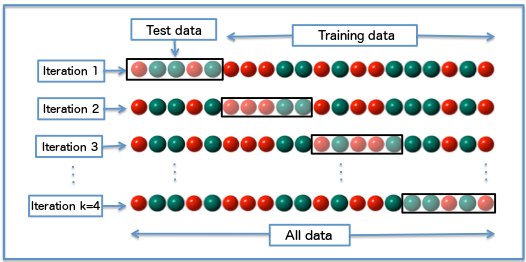
\includegraphics[width=1.0\textwidth]{figs/cv.jpg}
\caption{Visualization of a 4-fold CV. CC BY-SA 3.0 author Fabian Fl\"ock }
\end{figure}
\end{frame}

\begin{frame}{K-fold CV tips}
\begin{itemize}
\item In practice $k$ can be anywhere between 5-20
\item There is no best $k$
\item 10-fold CV is really common
\item everyone developes their own preference
\item Use for model validation
\item Use to approximate the accuracy of the model
\end{itemize}
\end{frame}

\begin{frame}[fragile]{Scikit-learn includes a KFold CV iterator}
Use KFold as a cross validation iterator.
\begin{minted}
{python}
from sklearn import svm
from sklearn import datasets
clf = svm.SVC()
iris = datasets.load_iris()
X, y = iris.data, iris.target

# import the cross validation iterator
from sklearn.model_selection import KFold
# initialize the KFold object for 5 fold CV
kf = KFold(n_splits=5)

for train, test in kf.split(X):
	# train are the indexes of the training set
	# test are the indexes of the test set
	X_test, X_train = X[test], X[train]
	y_test, y_train = y[test], y[train]
\end{minted}
\end{frame}

\begin{frame}[fragile]{Train and validate the model within each loop of the iteration}
\begin{minted}
{python}
score = []
for train, test in kf.split(X):
	# train are the indexes of the training set
	# test are the indexes of the test set
	X_test, X_train = X[test], X[train]
	y_test, y_train = y[test], y[train]
	
	# fit the model on the train set
	clf.fit(X_train,y_train)
	
	# score the model on the test set
	score.append(clf.score(X_test, y_test))

print('5 Fold CV avg score =', np.mean(score))
\end{minted}
\end{frame}

\begin{frame}[fragile]{Scikit-Learn includes a function to do this in one line}
If you have a bunch of models, and different pre-processing the KFold iterator may be more helpful. However if you just want to do a quick CV score you can use the cross\_validate function.
\begin{minted}
{python}
# import the cross_validate function
from sklearn.model_selection import cross_validate

# get the 10 fold cross validation scores
scores = cross_validate(clf, X, y,                         
        cv=10, return_train_score=False)
        
# this creates a dictionary of the scores
print('scores =', scores)

print('10 Fold CV avg score =', np.mean(scores['test_score']))
\end{minted}
\end{frame}


\begin{frame}{Cross validation and Scikit-learn summary}
\begin{itemize}
\item There are many model validation tools in Scikit-Learn
\item K-fold cross validation is useful for model validation
\item KFold is a cross validation model iterator
\item Alternatively there is a cross\_validate function to get the CV scores
\item General 5-fold to 20-fold cross validations are used
\end{itemize}
\end{frame}


\begin{frame}{scikit-learn comes with a few small standard datasets}
\textbf{Toy datasets} for practice
\begin{itemize}
\item load\_boston	Load and return the boston house-prices dataset (regression).
\item load\_iris	Load and return the iris dataset (classification).
\item load\_diabetes 	Load and return the diabetes dataset (regression).
\item load\_digits	Load and return the digits dataset (classification).
\item load\_linnerud 	Load and return the linnerud dataset (multivariate regression).
\item load\_wine 	Load and return the wine dataset (classification).
\item load\_breast\_cancer	Load and return the breast cancer wisconsin dataset (classification).
\end{itemize}
\end{frame}

\begin{frame}[fragile]{Scaling for zero mean and unit variance}
A lot of algorithms are sensitive to scaling (such as SVC) of the design features. Standard scalar mean centers you design features and scales for unit variance.
\begin{minted}
{python}
from sklearn.preprocessing import StandardScaler
import numpy as np
X_train = np.array([[ 1., -1.,  2.],
                    [ 2.,  0.,  0.],
                    [ 0.,  1., -1.]])
ss = StandardScaler()
# fit the pre-processing model to the training set
ss.fit(X_train)
# transform the training set
X_train = ss.transform(X_train)
print(X_train)
print('mean = ', np.mean(X_train,axis=0))
print('std = ', np.std(X_train,axis=0))

\end{minted}
\end{frame}

\begin{frame}{There are a number of example datasets in Documentation}
\url{http://scikit-learn.org/stable/auto_examples/index.html}
\end{frame}

\begin{frame}[fragile]{Nueral Network on MNIST dataset}
\begin{minted}
{python}
import matplotlib.pyplot as plt
from sklearn.datasets import fetch_mldata
from sklearn.neural_network import MLPClassifier
from sklearn.preprocessing import StandardScaler
mnist = fetch_mldata("MNIST original")
# rescale the data, use the traditional train/test split
X, y = mnist.data, mnist.target


# transform X for unit scaling
ss = StandardScaler()
X = ss.fit_transform(X)

# create test train set
X_train, X_test = X[:60000], X[60000:]
y_train, y_test = y[:60000], y[60000:]
\end{minted}
\end{frame}

\begin{frame}[fragile]{Nueral Network on MNIST dataset}
\begin{minted}
{python}
# set up my layers
layers = (256, 128, 64, 32, 16, 4)
# there will be two more layers than len(n)
# these are the number of nodes on hidden layers

# load MLP model
mlp = MLPClassifier(hidden_layer_sizes=layers, max_iter=1000, alpha=1e-4,
                solver='adam', verbose=10, tol=0, random_state=13,
                learning_rate='adaptive')
mlp.fit(X_train,y_train)

# score the  model
print(mlp.score(X_test,y_test))

# this only scores about 0.968
# if you want to learn more, check out the TF tutorial
# https://www.tensorflow.org/get_started/mnist/beginners
\end{minted}
\end{frame}

%\begin{frame}[fragile]{Quiz feedback}
%\begin{minted}
%{python}
%# let's consider an arbitrary function
%def my_fun():
%    return
%    
%# this won't execute the function, nor will it pass an error
%my_fun
%
%# infact I can even create an alias name of the function
%new = my_fun
%
%# again this won't execute the function
%new
%
%# You need to use () to execute a function
%new()
%\end{minted}
%\end{frame}
%
%\begin{frame}[fragile]{Quiz feedback plotting}
%\begin{minted}
%{python}
%import numpy as np
%import matplotlib.pyplot as plt
%
%x = np.linspace(0,20)
%y = 2.0*x - .3
%
%plt.figure()
%plt.plot(x,y)
%plt.show # this doesn't display the figure, 
%# it's just the name of the function!
%
%# you need to execute the function in order 
%# to display the figure
%plt.show()
%\end{minted}
%\end{frame}
%
%\begin{frame}{Topic for today: Scikit-Learn}
%\begin{itemize}
%\item    Simple and efficient tools for data mining and data analysis
%\item    Accessible to everybody, and reusable in various contexts
%\item    Built on NumPy, SciPy, and matplotlib
%\item    Open source, commercially usable - BSD license
%\end{itemize}
%
%Dr. Jake VanderPlas’s Python Data Science
%Handbook: Essential Tools for Working with Data. \url{http://shop.oreilly.com/product/0636920034919.do}
%
%The textbook available for free in the form of Jupyter notebooks which
%can be viewed at \url{https://github.com/jakevdp/PythonDataScienceHandbook}  or \url{http://nbviewer.jupyter.org/github/jakevdp/PythonDataScienceHandbook/blob/master/notebooks/Index.ipynb}
%\end{frame}
%
%\begin{frame}{Scikit-Learn has great documentation}
%with plenty of tutorials and examples for each class... You should take a look at it
%
%\url{http://scikit-learn.org/}
%
%\end{frame}
%
%\begin{frame}{What is classification? - Supervised learning}
%\begin{itemize}
%\item Given a collection of labeled features: Can we find a pattern in the features to predict the labels?
%\item Classification is used everywhere!
%\item Ex: You are applying for a loan. The bank knows your income, job stability, and debt. Are you approved for the load?
%\item Features: income, job stability, debt
%\item Labels: approve or reject
%\item Binary classification problem!
%\end{itemize}
%\end{frame}
%
%\begin{frame}{New iPhone X - unlock with your face}
%\begin{figure}
%
\includegraphics[width=1.0\textwidth]{figs/iphonex.png}
%\end{figure}
%\end{frame}
%
%\begin{frame}{Classification example 1}
%\begin{figure}
%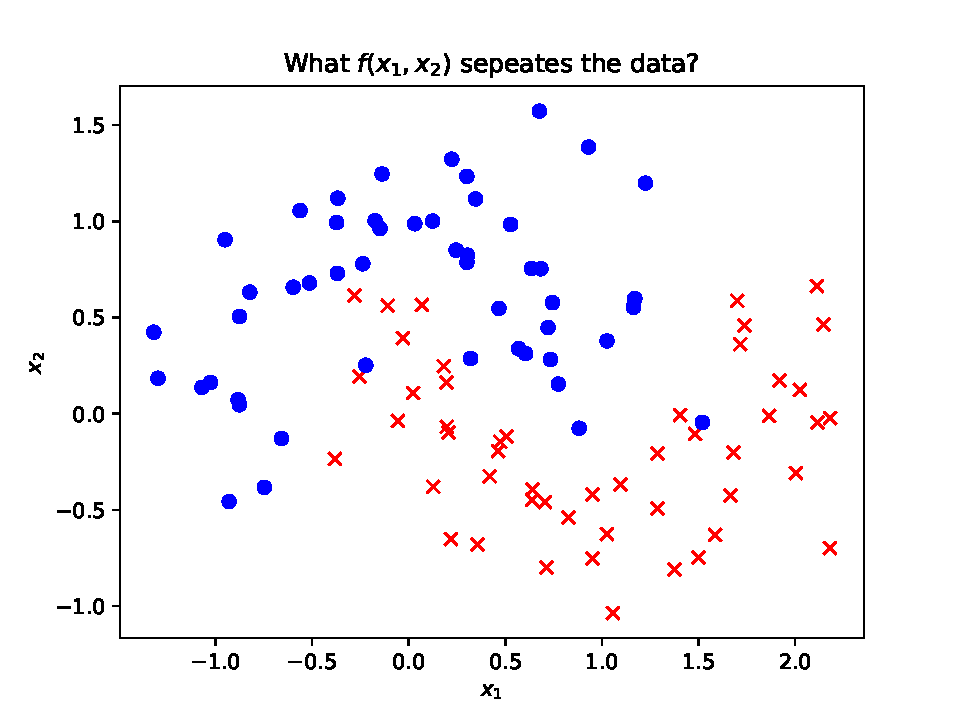
\includegraphics[width=1.0\textwidth]{figs/1.pdf}
%\end{figure}
%\end{frame}
%
%\begin{frame}{Classification example 2}
%\begin{figure}
%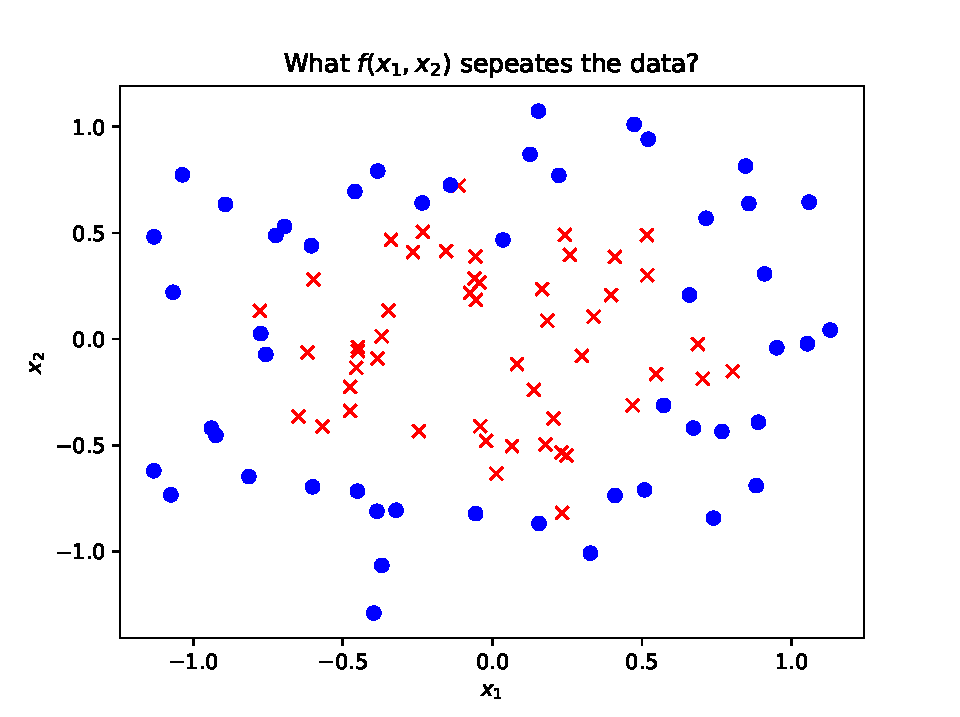
\includegraphics[width=1.0\textwidth]{figs/2.pdf}
%\end{figure}
%\end{frame}
%
%\begin{frame}{Classification example 3}
%\begin{figure}
%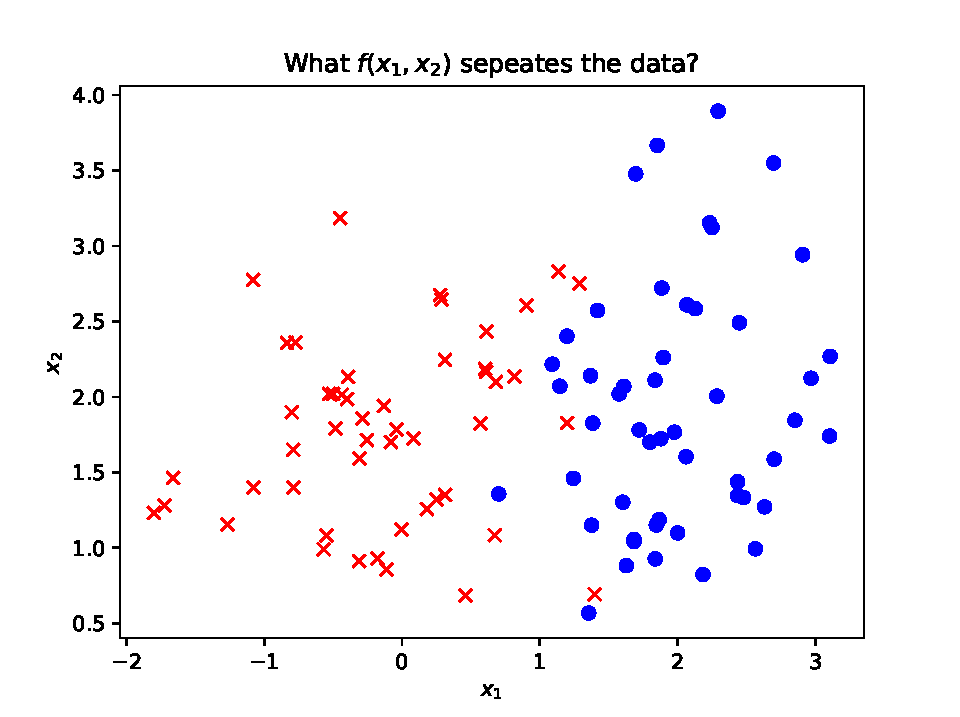
\includegraphics[width=1.0\textwidth]{figs/3.pdf}
%\end{figure}
%\end{frame}
%
%\begin{frame}{What is regression? }
%\begin{itemize}
%\item Can we find the trend in data?
%\item Can we predict the values in-between data points? 
%\item Classification is used everywhere!
%\item Ex: You are applying for a loan. The bank knows your income, job stability, and debt. How much of a loan can you get approved for?
%\item Variables: income, job stability, debt
%\item Output: How much \$ you get?
%\end{itemize}
%\end{frame}
%
%\begin{frame}{Linear regression: fitting a line to data}
%\begin{figure}
%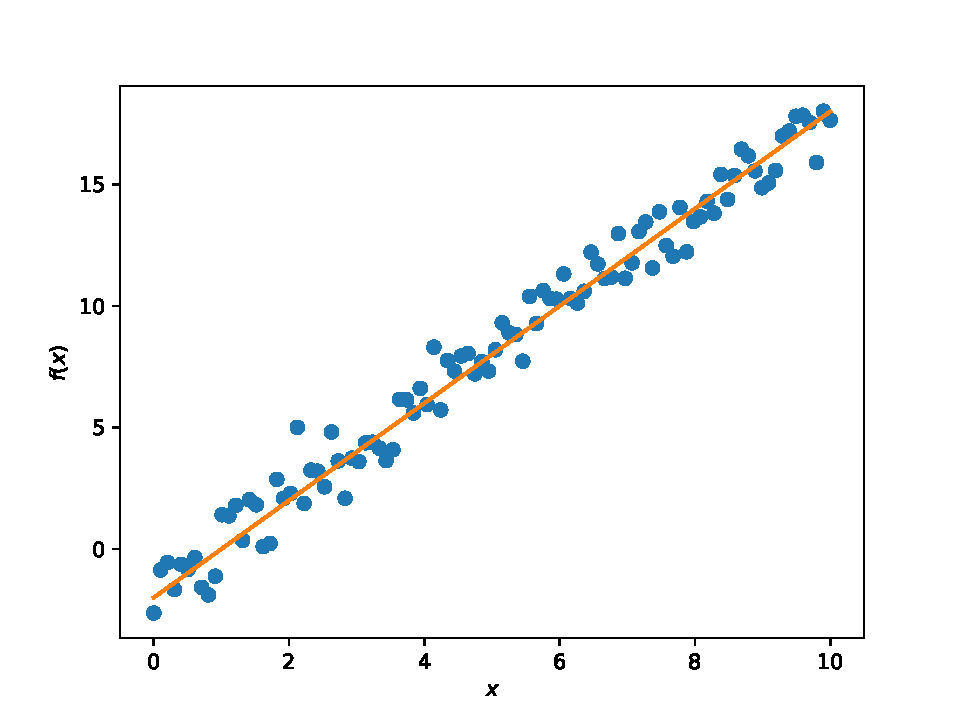
\includegraphics[width=1.0\textwidth]{figs/linear_regression.pdf}
%\end{figure}
%\end{frame}
%
%\begin{frame}{Kriging: using correlation between data}
%\begin{figure}
%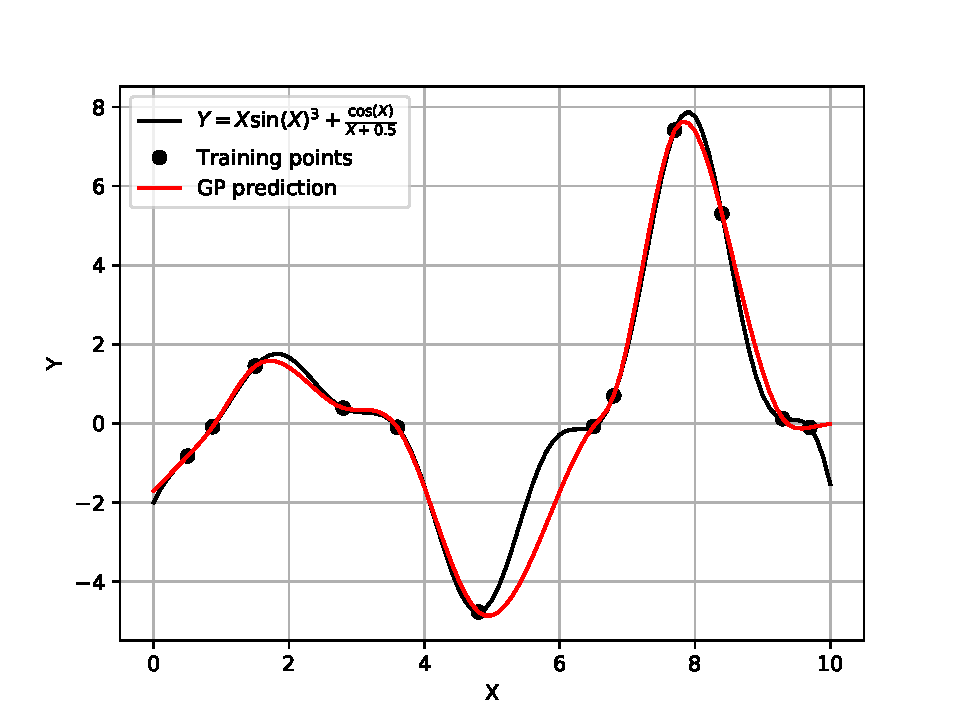
\includegraphics[width=1.0\textwidth]{figs/Kriging.pdf}
%\end{figure}
%\end{frame}
%
%\begin{frame}{What is clustering? Unsupervised learning}
%\begin{itemize}
%\item Can we find the structure in data?
%\item Can we detect and identify groups in data?
%\item Ex: We have a bunch of data related to income, job stability, and debt. Can we identify a pattern in the data?
%\item The key is that we don't know the label or value. 
%\item Ex: Used to identify similarities in protein chains 
%\end{itemize}
%\end{frame}
%
%\begin{frame}{Clustering: Can we categorize this data?}
%\begin{figure}
%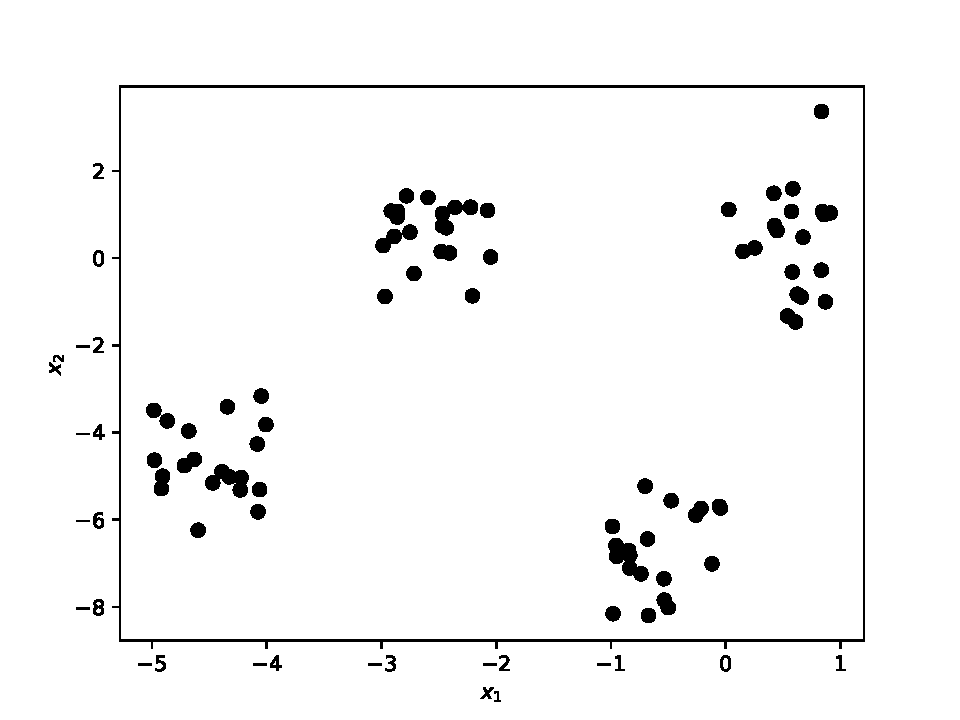
\includegraphics[width=1.0\textwidth]{figs/clust.pdf}
%\end{figure}
%\end{frame}
%
%\begin{frame}{Clustering output}
%\begin{figure}
%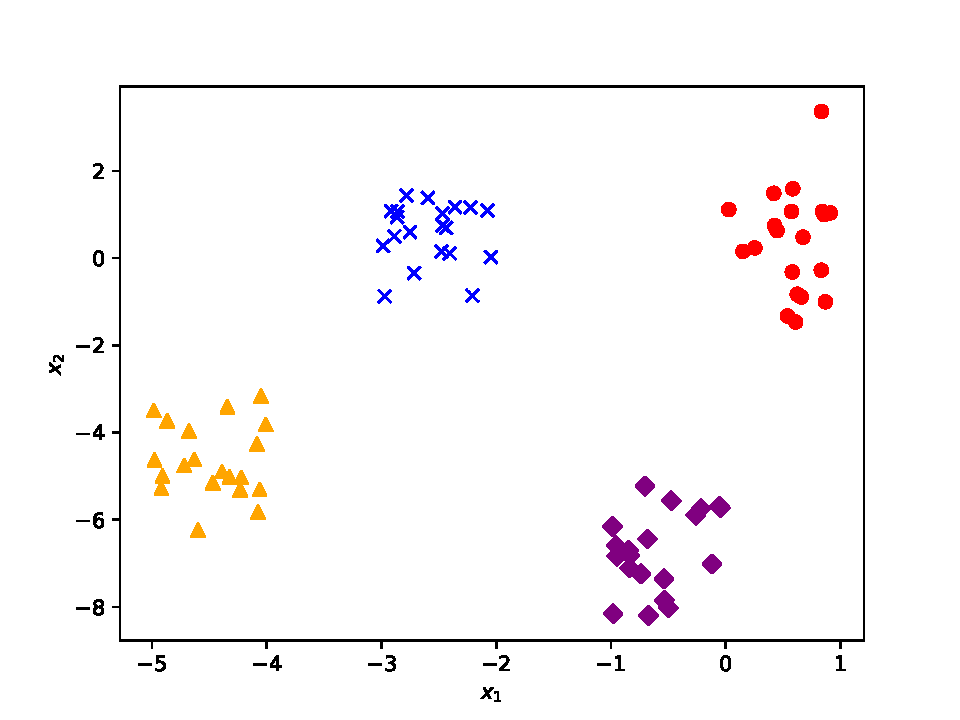
\includegraphics[width=1.0\textwidth]{figs/cluster.pdf}
%\end{figure}
%\end{frame}
%
%\begin{frame}{So what does the data look like for Scikit-Learn}
%Out input data will be a matrix (or numpy array) with $n$ number of samples and $d$ number of design variables (or \textbf{features})
%\begin{equation}
%\bm{X} = \begin{bmatrix}
%x_{11} & x_{12} & x_{13} & \cdots & x_{1d} \\ 
%x_{21} & x_{22} & x_{23} & \cdots & x_{2d} \\ 
%x_{31} & x_{32} & x_{33} & \cdots & x_{3d} \\ 
%\vdots & \vdots * \vdots & \vdots & \vdots \\
%x_{n1} & x_{n2} & x_{n3} & \cdots & x_{nd} \\ 
%\end{bmatrix}
%\end{equation}
%Each row of $\bm{X}$ represents a single sample.
%
%
%Out output data will be a vector $\bm{y}$ (usually a numpy array) with $n$ number samples.
%\begin{equation}
%\bm{y} = \begin{bmatrix}
%y_{1} \\
%y_{2} \\
%y_{3} \\
%\vdots \\
%y_{n} \\
%\end{bmatrix}
%\end{equation}
%\end{frame}
%
%\begin{frame}[fragile]{Let's consider a simple linear regression example}
%\begin{minted}
%{python}
%import numpy as np
%import matplotlib.pyplot as plt
%
%# let's create some arbitrary data
%# and fit a line to it
%
%np.random.seed(33)
%x = 10.0*np.random.random(100)
%noise = np.random.normal(loc=0.5, size=100)
%y = 2.3*x - 3 + noise
%plt.figure()
%plt.plot(X,y, 'o')
%plt.show()
%\end{minted}
%\end{frame}
%
%\begin{frame}[fragile]{Building a linear regression model}
%\begin{minted}
%{python}
%from sklearn.linear_model import LinearRegression
%# LinearRegression is a Python class that we'll use to create
%# our linear model object
%
%# we can't pass a vector into scikit-learn
%# instead we need to pass a feature matrix
%# we can do this by reshaping x
%X = x.reshape(-1,1)
%
%# we initialize a model object from the LinearRegression class
%# to begin the process. With the initialization, we can pass
%# model hyper-parameters, in this case we pass that a 
%# y intercept be determined
%model = LinearRegression(fit_intercept=True)
%\end{minted}
%\end{frame}
%
%\begin{frame}[fragile]{Fitting the linear regression model}
%\begin{minted}
%{python}
%# simply pass your training data into the model's fit function
%# which will run an 'optimization' selecting the best parameters
%# == this is the same as an ordinary least squares fit ==
%model.fit(X,y)
%
%# in this case there are two parameters for the line 
%# y = mx + b
%print('m = ', model.coef_)
%print('b = ', model.intercept_)
%# score calculates the R^2 (Coefficient of determination) 
%# for a given input and output 
%my_score = model.score(X,y)
%
%print('R^2 = ', my_score)
%\end{minted}
%\end{frame}
%
%\begin{frame}[fragile]{Predicting for new $x$ values}
%\begin{minted}
%{python}
%# let's generate new x values from slightly smaller than min(x)
%# to the slightly larger than the max(x)
%x_hat = np.linspace(np.min(x)-1.0,  np.max(x)+1.0, 100)
%
%# Again x_hat is a vector, and must be reshaped 
%# to be a 2 dimensional array
%X_hat = x_hat.reshape(-1, 1)
%
%# we can find new y_hat values by using the model.predict function
%y_hat = model.predict(X_hat)
%
%# let's plot the results
%plt.figure()
%plt.plot(X,y, 'o')
%plt.plot(x_hat, y_hat, '-')
%plt.show()
%\end{minted}
%\end{frame}
%
%\begin{frame}[fragile]{What about polynomials?}
%So let's consider a toy polynomial problem where
%\begin{equation}
%y = \beta_0 + \beta_1 x + \beta_2 x^2
%\end{equation}
%on the domain $-10.0 \leq x \leq 10.0$
%
%\begin{minted}
%{python}
%# generate artificial data
%np.random.seed(19)
%x = (10.0 + 10.0)* np.random.random(100) - 10.0
%noise = np.random.normal(scale=5.0,size=100)
%y = -1.0 + 2.2*x - 0.5*x**2 + noise
%
%plt.figure()
%plt.plot(x,y, 'o')
%plt.show()
%\end{minted}
%\end{frame}
%
%\begin{frame}[fragile]{Scikit-Learn includes a polynomial prepossessing tool}
%So in order the least squares regression, we need to construct the regression matrix $\bm{X}$. Scikit-Learn includes a Polynomial class for doing this easily.
%\begin{minted}
%{python}
%from sklearn.preprocessing import PolynomialFeatures
%# again we need to transfer x to a matrix... 
%# the reason is that sklearn doesn't deal with 1D data...
%X = x.reshape(-1,1)
%
%# create a poly object from the PolynomialFeatures class
%# in our case we'll be fitting a second order polynomial
%poly = PolynomialFeatures(degree=2)
%
%# now we use poly to transform our X into a Regression matrix!
%X = poly.fit_transform(X)
%print(X)
%# note this transformation includes the y intercept!
%\end{minted}
%\end{frame}
%
%\begin{frame}[fragile]{Fitting the second order polynomial}
%\begin{minted}
%{python}
%# create quad object from linear regression
%# the default is that fit_intercept = False
%# we don't want fit_intercept because it's included in X
%quad = LinearRegression(fit_intercept=False)
%
%# perform the least squares fit
%quad.fit(X,y)
%
%# predict for new values of x
%x_hat = np.linspace(np.min(x), np.max(x), 100)
%x_hat = x_hat.reshape(-1,1)
%X_hat = poly.fit_transform(x_hat)
%y_hat = quad.predict(X_hat)
%
%# plot the results
%plt.figure()
%plt.plot(x,y, 'o')
%plt.plot(x_hat, y_hat, '-')
%plt.show()
%\end{minted}
%\end{frame}
%
%\begin{frame}[fragile]{What are the resulting parameters?}
%Recall \begin{equation}
%y = \beta_0 + \beta_1 x + \beta_2 x^2
%\end{equation}
%
%You $\beta$ parameters are stored in the quad object.
%\begin{minted}
%{python}
%print('beta0 =', quad.coef_[0])
%print('beta1 =', quad.coef_[1])
%print('beta2 =', quad.coef_[2])
%\end{minted}
%\end{frame}
%
%\begin{frame}[fragile]{What about polynomials for higher dimensions?}
%Consider a polynomial response surface\begin{equation}
%f(x_1,x_2) = \beta_0 + \beta_1 x_1 + \beta_2x_2 + \beta_3x_1^2 + \beta_4x_1x_2 + \beta_5x_2^2
%\end{equation}
%\begin{minted}
%{python}
%# let's generate a 2 dimensional polynomial problem
%np.random.seed(121)
%X = np.random.random((100,2))
%# since this is a matrix, there is no need to reshape
%y = 1.0 + X[:,0] + 0.9*X[:,1] + 1.2*X[:,0]**2  \
%-1.3*X[:,0]*X[:,1] - 3.0*X[:,1]**2
%# plot the data
%from mpl_toolkits.mplot3d import Axes3D
%import matplotlib.pyplot as plt
%fig = plt.figure()
%ax = fig.add_subplot(111, projection='3d')
%ax.scatter(X[:,0], X[:,1], y, 'o')
%ax.set(xlabel='$x_1$', ylabel='$x_2$', zlabel='$f(x_1,x_2$')
%fig.show()
%\end{minted}
%\end{frame}
%
%\begin{frame}[fragile]{Same process for creating regression matrix and fitting}
%\begin{minted}
%{python}
%from sklearn.preprocessing import PolynomialFeatures
%poly = PolynomialFeatures(degree=2)
%X_train = poly.fit_transform(X)
%
%
%# fit the model
%model = LinearRegression(fit_intercept=False)
%model.fit(X_train,y)
%# print the model coefficients - you'll see they are exact!
%print(model.coef_)
%
%# Let's generate sampeles to predict over the domain
%x = np.linspace(np.min(X), np.max(X), 10)
%x1,x2 = np.meshgrid(x,x)
%X_hat = np.zeros((100,2))
%X_hat[:,0] = x1.flatten()
%X_hat[:,1] = x2.flatten()
%\end{minted}
%\end{frame}
%
%\begin{frame}[fragile]{Predicting and comparing the result}
%\begin{minted}
%{python}
%X_test = poly.fit_transform(X_hat)
%
%# predict for X_test
%Y_hat = model.predict(X_test)
%
%# reshape y_hat
%y_hat = Y_hat.reshape((10,10))
%
%# plot the results
%fig = plt.figure()
%ax = fig.add_subplot(111, projection='3d')
%ax.plot_surface(x1, x2, y_hat)
%ax.scatter(X[:,0], X[:,1], y, 'o', color='black')
%ax.set(xlabel='$x_1$', ylabel='$x_2$', zlabel='$f(x_1,x_2$')
%fig.show()
%\end{minted}
%\end{frame}
%
%\begin{frame}[fragile]{Classifcation with the famous flower database...}
%Naive Bayes Classification of Iris dataset...
%\begin{minted}
%{python}
%import seaborn as sns
%iris = sns.load_dataset('iris')
%
%X_iris = iris.drop('species', axis=1)
%y_iris = iris['species']  
%
%# sklearn includes tools for validation and model selection
%from sklearn.cross_validation import train_test_split
%Xtrain, Xtest, ytrain, ytest = train_test_split(X_iris, y_iris, random_state=1)   
%# this code splits the entire dataset into two
%# a training set and a testing set
%\end{minted}
%
%\end{frame}
%
%\begin{frame}[fragile]{The process for fitting models is same: apply NB}
%\begin{minted}
%{python}
%# 1. choose model class
%from sklearn.naive_bayes import GaussianNB 
%
%# 2. instantiate model
%model = GaussianNB()  
%   
%# 3. fit model to data                  
%model.fit(Xtrain, ytrain)   
%
%# 4. predict on new data                
%y_hat = model.predict(Xtest)
%
%# 5. score the model
%print(model.score(Xtest,ytest))          
%\end{minted}
%\end{frame}



\end{document}
